\documentclass[twoside]{book}

% Packages required by doxygen
\usepackage{fixltx2e}
\usepackage{calc}
\usepackage{doxygen}
\usepackage[export]{adjustbox} % also loads graphicx
\usepackage{graphicx}
\usepackage[utf8]{inputenc}
\usepackage{makeidx}
\usepackage{multicol}
\usepackage{multirow}
\PassOptionsToPackage{warn}{textcomp}
\usepackage{textcomp}
\usepackage[nointegrals]{wasysym}
\usepackage[table]{xcolor}

% Font selection
\usepackage[T1]{fontenc}
\usepackage[scaled=.90]{helvet}
\usepackage{courier}
\usepackage{amssymb}
\usepackage{sectsty}
\renewcommand{\familydefault}{\sfdefault}
\allsectionsfont{%
  \fontseries{bc}\selectfont%
  \color{darkgray}%
}
\renewcommand{\DoxyLabelFont}{%
  \fontseries{bc}\selectfont%
  \color{darkgray}%
}
\newcommand{\+}{\discretionary{\mbox{\scriptsize$\hookleftarrow$}}{}{}}

% Page & text layout
\usepackage{geometry}
\geometry{%
  a4paper,%
  top=2.5cm,%
  bottom=2.5cm,%
  left=2.5cm,%
  right=2.5cm%
}
\tolerance=750
\hfuzz=15pt
\hbadness=750
\setlength{\emergencystretch}{15pt}
\setlength{\parindent}{0cm}
\setlength{\parskip}{0.2cm}
\makeatletter
\renewcommand{\paragraph}{%
  \@startsection{paragraph}{4}{0ex}{-1.0ex}{1.0ex}{%
    \normalfont\normalsize\bfseries\SS@parafont%
  }%
}
\renewcommand{\subparagraph}{%
  \@startsection{subparagraph}{5}{0ex}{-1.0ex}{1.0ex}{%
    \normalfont\normalsize\bfseries\SS@subparafont%
  }%
}
\makeatother

% Headers & footers
\usepackage{fancyhdr}
\pagestyle{fancyplain}
\fancyhead[LE]{\fancyplain{}{\bfseries\thepage}}
\fancyhead[CE]{\fancyplain{}{}}
\fancyhead[RE]{\fancyplain{}{\bfseries\leftmark}}
\fancyhead[LO]{\fancyplain{}{\bfseries\rightmark}}
\fancyhead[CO]{\fancyplain{}{}}
\fancyhead[RO]{\fancyplain{}{\bfseries\thepage}}
\fancyfoot[LE]{\fancyplain{}{}}
\fancyfoot[CE]{\fancyplain{}{}}
\fancyfoot[RE]{\fancyplain{}{\bfseries\scriptsize Generated on Fri Jul 24 2015 11\+:38\+:22 for Post\+G\+I\+S\+Helpers by Doxygen }}
\fancyfoot[LO]{\fancyplain{}{\bfseries\scriptsize Generated on Fri Jul 24 2015 11\+:38\+:22 for Post\+G\+I\+S\+Helpers by Doxygen }}
\fancyfoot[CO]{\fancyplain{}{}}
\fancyfoot[RO]{\fancyplain{}{}}
\renewcommand{\footrulewidth}{0.4pt}
\renewcommand{\chaptermark}[1]{%
  \markboth{#1}{}%
}
\renewcommand{\sectionmark}[1]{%
  \markright{\thesection\ #1}%
}

% Indices & bibliography
\usepackage{natbib}
\usepackage[titles]{tocloft}
\setcounter{tocdepth}{3}
\setcounter{secnumdepth}{5}
\makeindex

% Hyperlinks (required, but should be loaded last)
\usepackage{ifpdf}
\ifpdf
  \usepackage[pdftex,pagebackref=true]{hyperref}
\else
  \usepackage[ps2pdf,pagebackref=true]{hyperref}
\fi
\hypersetup{%
  colorlinks=true,%
  linkcolor=blue,%
  citecolor=blue,%
  unicode%
}

% Custom commands
\newcommand{\clearemptydoublepage}{%
  \newpage{\pagestyle{empty}\cleardoublepage}%
}


%===== C O N T E N T S =====

\begin{document}

% Titlepage & ToC
\hypersetup{pageanchor=false,
             bookmarks=true,
             bookmarksnumbered=true,
             pdfencoding=unicode
            }
\pagenumbering{roman}
\begin{titlepage}
\vspace*{7cm}
\begin{center}%
{\Large Post\+G\+I\+S\+Helpers \\[1ex]\large 0.\+1 }\\
\vspace*{1cm}
{\large Generated by Doxygen 1.8.10}\\
\vspace*{0.5cm}
{\small Fri Jul 24 2015 11:38:22}\\
\end{center}
\end{titlepage}
\clearemptydoublepage
\tableofcontents
\clearemptydoublepage
\pagenumbering{arabic}
\hypersetup{pageanchor=true}

%--- Begin generated contents ---
\chapter{rli\+\_\+python\+\_\+as\+\_\+gis}
\label{md___users_blubber__documents__software_dev__workspace__python__projects_rli_python_as_gis__r_e_a_d_m_e}
\hypertarget{md___users_blubber__documents__software_dev__workspace__python__projects_rli_python_as_gis__r_e_a_d_m_e}{}
Set of files used to explore Python\textquotesingle{}s G\+I\+S capabilities 
\chapter{Namespace Index}
\section{Namespace List}
Here is a list of all documented namespaces with brief descriptions\+:\begin{DoxyCompactList}
\item\contentsline{section}{\hyperlink{namespace_post_g_i_s_helpers}{Post\+G\+I\+S\+Helpers} }{\pageref{namespace_post_g_i_s_helpers}}{}
\item\contentsline{section}{\hyperlink{namespace_web_o_s_m_helpers}{Web\+O\+S\+M\+Helpers} }{\pageref{namespace_web_o_s_m_helpers}}{}
\end{DoxyCompactList}

\chapter{Hierarchical Index}
\section{Class Hierarchy}
This inheritance list is sorted roughly, but not completely, alphabetically\+:\begin{DoxyCompactList}
\item \contentsline{section}{S\+Q\+L\+Operations.\+D\+B\+Operations}{\pageref{class_s_q_l_operations_1_1_d_b_operations}}{}
\item \contentsline{section}{Post\+G\+I\+S\+Helpers.\+Query}{\pageref{class_post_g_i_s_helpers_1_1_query}}{}
\begin{DoxyCompactList}
\item \contentsline{section}{Post\+G\+I\+S\+Helpers.\+Lines}{\pageref{class_post_g_i_s_helpers_1_1_lines}}{}
\begin{DoxyCompactList}
\item \contentsline{section}{Post\+G\+I\+S\+Helpers.\+O\+S\+M\+Lines}{\pageref{class_post_g_i_s_helpers_1_1_o_s_m_lines}}{}
\end{DoxyCompactList}
\item \contentsline{section}{Post\+G\+I\+S\+Helpers.\+O\+S\+M\+Query}{\pageref{class_post_g_i_s_helpers_1_1_o_s_m_query}}{}
\begin{DoxyCompactList}
\item \contentsline{section}{Post\+G\+I\+S\+Helpers.\+O\+S\+M\+Collection}{\pageref{class_post_g_i_s_helpers_1_1_o_s_m_collection}}{}
\item \contentsline{section}{Post\+G\+I\+S\+Helpers.\+O\+S\+M\+Lines}{\pageref{class_post_g_i_s_helpers_1_1_o_s_m_lines}}{}
\item \contentsline{section}{Post\+G\+I\+S\+Helpers.\+O\+S\+M\+Points}{\pageref{class_post_g_i_s_helpers_1_1_o_s_m_points}}{}
\item \contentsline{section}{Post\+G\+I\+S\+Helpers.\+O\+S\+M\+Polygons}{\pageref{class_post_g_i_s_helpers_1_1_o_s_m_polygons}}{}
\end{DoxyCompactList}
\item \contentsline{section}{Post\+G\+I\+S\+Helpers.\+Points}{\pageref{class_post_g_i_s_helpers_1_1_points}}{}
\begin{DoxyCompactList}
\item \contentsline{section}{Post\+G\+I\+S\+Helpers.\+O\+S\+M\+Points}{\pageref{class_post_g_i_s_helpers_1_1_o_s_m_points}}{}
\end{DoxyCompactList}
\item \contentsline{section}{Post\+G\+I\+S\+Helpers.\+Polygons}{\pageref{class_post_g_i_s_helpers_1_1_polygons}}{}
\begin{DoxyCompactList}
\item \contentsline{section}{Post\+G\+I\+S\+Helpers.\+O\+S\+M\+Polygons}{\pageref{class_post_g_i_s_helpers_1_1_o_s_m_polygons}}{}
\end{DoxyCompactList}
\end{DoxyCompactList}
\item \contentsline{section}{region.\+Region}{\pageref{classregion_1_1_region}}{}
\item \contentsline{section}{simple\+\_\+log.\+Simple\+Logger}{\pageref{classsimple__log_1_1_simple_logger}}{}
\end{DoxyCompactList}

\chapter{Class Index}
\section{Class List}
Here are the classes, structs, unions and interfaces with brief descriptions\+:\begin{DoxyCompactList}
\item\contentsline{section}{\hyperlink{class_s_q_l_operations_1_1_d_b_operations}{S\+Q\+L\+Operations.\+D\+B\+Operations} }{\pageref{class_s_q_l_operations_1_1_d_b_operations}}{}
\item\contentsline{section}{\hyperlink{class_post_g_i_s_helpers_1_1_lines}{Post\+G\+I\+S\+Helpers.\+Lines} }{\pageref{class_post_g_i_s_helpers_1_1_lines}}{}
\item\contentsline{section}{\hyperlink{class_post_g_i_s_helpers_1_1_o_s_m_collection}{Post\+G\+I\+S\+Helpers.\+O\+S\+M\+Collection} }{\pageref{class_post_g_i_s_helpers_1_1_o_s_m_collection}}{}
\item\contentsline{section}{\hyperlink{class_post_g_i_s_helpers_1_1_o_s_m_lines}{Post\+G\+I\+S\+Helpers.\+O\+S\+M\+Lines} }{\pageref{class_post_g_i_s_helpers_1_1_o_s_m_lines}}{}
\item\contentsline{section}{\hyperlink{class_post_g_i_s_helpers_1_1_o_s_m_points}{Post\+G\+I\+S\+Helpers.\+O\+S\+M\+Points} }{\pageref{class_post_g_i_s_helpers_1_1_o_s_m_points}}{}
\item\contentsline{section}{\hyperlink{class_post_g_i_s_helpers_1_1_o_s_m_polygons}{Post\+G\+I\+S\+Helpers.\+O\+S\+M\+Polygons} }{\pageref{class_post_g_i_s_helpers_1_1_o_s_m_polygons}}{}
\item\contentsline{section}{\hyperlink{class_post_g_i_s_helpers_1_1_o_s_m_query}{Post\+G\+I\+S\+Helpers.\+O\+S\+M\+Query} }{\pageref{class_post_g_i_s_helpers_1_1_o_s_m_query}}{}
\item\contentsline{section}{\hyperlink{class_post_g_i_s_helpers_1_1_points}{Post\+G\+I\+S\+Helpers.\+Points} }{\pageref{class_post_g_i_s_helpers_1_1_points}}{}
\item\contentsline{section}{\hyperlink{class_post_g_i_s_helpers_1_1_polygons}{Post\+G\+I\+S\+Helpers.\+Polygons} }{\pageref{class_post_g_i_s_helpers_1_1_polygons}}{}
\item\contentsline{section}{\hyperlink{class_post_g_i_s_helpers_1_1_query}{Post\+G\+I\+S\+Helpers.\+Query} }{\pageref{class_post_g_i_s_helpers_1_1_query}}{}
\item\contentsline{section}{\hyperlink{classregion_1_1_region}{region.\+Region} }{\pageref{classregion_1_1_region}}{}
\item\contentsline{section}{\hyperlink{classsimple__log_1_1_simple_logger}{simple\+\_\+log.\+Simple\+Logger} }{\pageref{classsimple__log_1_1_simple_logger}}{}
\end{DoxyCompactList}

\chapter{Namespace Documentation}
\hypertarget{namespace_post_g_i_s_helpers}{}\section{Post\+G\+I\+S\+Helpers Namespace Reference}
\label{namespace_post_g_i_s_helpers}\index{Post\+G\+I\+S\+Helpers@{Post\+G\+I\+S\+Helpers}}
\subsection*{Classes}
\begin{DoxyCompactItemize}
\item 
class \hyperlink{class_post_g_i_s_helpers_1_1_lines}{Lines}
\item 
class \hyperlink{class_post_g_i_s_helpers_1_1_o_s_m_collection}{O\+S\+M\+Collection}
\item 
class \hyperlink{class_post_g_i_s_helpers_1_1_o_s_m_lines}{O\+S\+M\+Lines}
\item 
class \hyperlink{class_post_g_i_s_helpers_1_1_o_s_m_points}{O\+S\+M\+Points}
\item 
class \hyperlink{class_post_g_i_s_helpers_1_1_o_s_m_polygons}{O\+S\+M\+Polygons}
\item 
class \hyperlink{class_post_g_i_s_helpers_1_1_o_s_m_query}{O\+S\+M\+Query}
\item 
class \hyperlink{class_post_g_i_s_helpers_1_1_points}{Points}
\item 
class \hyperlink{class_post_g_i_s_helpers_1_1_polygons}{Polygons}
\item 
class \hyperlink{class_post_g_i_s_helpers_1_1_query}{Query}
\end{DoxyCompactItemize}
\subsection*{Variables}
\begin{DoxyCompactItemize}
\item 
\hypertarget{namespace_post_g_i_s_helpers_a35221781bcc71b63ef13db443ee5290b}{}tuple {\bfseries logger} = \hyperlink{classsimple__log_1_1_simple_logger}{Simple\+Logger}(module\+\_\+name=\char`\"{}Post\+G\+I\+S\+Helpers\char`\"{})\label{namespace_post_g_i_s_helpers_a35221781bcc71b63ef13db443ee5290b}

\end{DoxyCompactItemize}


\subsection{Detailed Description}
\begin{DoxyVerb}Requirements:

* Python3
* Matplotlib with Basemap-support (http://matplotlib.org/basemap/)

Package containing various methods for conveniently receiving and visualising
geoinformation from a PostGIS/Postgresql database or web services providing
openstreetmap data

Study usage_examples.py for some working examples (apply to your local database
infrastructure!)
\end{DoxyVerb}
 
\hypertarget{namespace_web_o_s_m_helpers}{}\section{Web\+O\+S\+M\+Helpers Namespace Reference}
\label{namespace_web_o_s_m_helpers}\index{Web\+O\+S\+M\+Helpers@{Web\+O\+S\+M\+Helpers}}
\subsection*{Functions}
\begin{DoxyCompactItemize}
\item 
def \hyperlink{namespace_web_o_s_m_helpers_a4bc15fc784f2d073a1a92fd90edaa446}{fetch\+\_\+admin\+\_\+from\+\_\+latlon} (lat, lon)
\end{DoxyCompactItemize}


\subsection{Detailed Description}
\begin{DoxyVerb}Set of small tools for querying OSM web services
\end{DoxyVerb}
 

\subsection{Function Documentation}
\hypertarget{namespace_web_o_s_m_helpers_a4bc15fc784f2d073a1a92fd90edaa446}{}\index{Web\+O\+S\+M\+Helpers@{Web\+O\+S\+M\+Helpers}!fetch\+\_\+admin\+\_\+from\+\_\+latlon@{fetch\+\_\+admin\+\_\+from\+\_\+latlon}}
\index{fetch\+\_\+admin\+\_\+from\+\_\+latlon@{fetch\+\_\+admin\+\_\+from\+\_\+latlon}!Web\+O\+S\+M\+Helpers@{Web\+O\+S\+M\+Helpers}}
\subsubsection[{fetch\+\_\+admin\+\_\+from\+\_\+latlon(lat, lon)}]{\setlength{\rightskip}{0pt plus 5cm}def Web\+O\+S\+M\+Helpers.\+fetch\+\_\+admin\+\_\+from\+\_\+latlon (
\begin{DoxyParamCaption}
\item[{}]{lat, }
\item[{}]{lon}
\end{DoxyParamCaption}
)}\label{namespace_web_o_s_m_helpers_a4bc15fc784f2d073a1a92fd90edaa446}
\begin{DoxyVerb}Receive geo information from lat/lon point (reverse geocoding)
:rtype : dict
:param lat: latitude
:param lon: longitude
:param zoom: detail level of information
:return: dictionary
\end{DoxyVerb}
 
\chapter{Class Documentation}
\hypertarget{class_s_q_l_operations_1_1_d_b_operations}{}\section{S\+Q\+L\+Operations.\+D\+B\+Operations Class Reference}
\label{class_s_q_l_operations_1_1_d_b_operations}\index{S\+Q\+L\+Operations.\+D\+B\+Operations@{S\+Q\+L\+Operations.\+D\+B\+Operations}}
\subsection*{Public Member Functions}
\begin{DoxyCompactItemize}
\item 
\hypertarget{class_s_q_l_operations_1_1_d_b_operations_a3f0d8876701395a42ff45f7b79c75d74}{}def {\bfseries \+\_\+\+\_\+enter\+\_\+\+\_\+} (self)\label{class_s_q_l_operations_1_1_d_b_operations_a3f0d8876701395a42ff45f7b79c75d74}

\item 
\hypertarget{class_s_q_l_operations_1_1_d_b_operations_a6740565be31768854cf36a3811e788a3}{}def {\bfseries \+\_\+\+\_\+init\+\_\+\+\_\+}\label{class_s_q_l_operations_1_1_d_b_operations_a6740565be31768854cf36a3811e788a3}

\item 
\hypertarget{class_s_q_l_operations_1_1_d_b_operations_a5a75d33811f72f5ab56ebb53b7744fa3}{}def {\bfseries execute\+\_\+query} (self, query)\label{class_s_q_l_operations_1_1_d_b_operations_a5a75d33811f72f5ab56ebb53b7744fa3}

\item 
\hypertarget{class_s_q_l_operations_1_1_d_b_operations_afe57de4264a7f52b4127308642aa4afd}{}def {\bfseries \+\_\+\+\_\+exit\+\_\+\+\_\+} (self, exc\+\_\+type, exc\+\_\+val, exc\+\_\+tb)\label{class_s_q_l_operations_1_1_d_b_operations_afe57de4264a7f52b4127308642aa4afd}

\end{DoxyCompactItemize}
\subsection*{Public Attributes}
\begin{DoxyCompactItemize}
\item 
\hypertarget{class_s_q_l_operations_1_1_d_b_operations_ab5d8122feb38fd555eb06c938b6a83db}{}{\bfseries connection}\label{class_s_q_l_operations_1_1_d_b_operations_ab5d8122feb38fd555eb06c938b6a83db}

\item 
\hypertarget{class_s_q_l_operations_1_1_d_b_operations_a93a542318dcdc666cae23196662a7e17}{}{\bfseries cur}\label{class_s_q_l_operations_1_1_d_b_operations_a93a542318dcdc666cae23196662a7e17}

\item 
\hypertarget{class_s_q_l_operations_1_1_d_b_operations_aa726a4bbd72110c98c27aa32f4c69c52}{}{\bfseries db\+\_\+setup}\label{class_s_q_l_operations_1_1_d_b_operations_aa726a4bbd72110c98c27aa32f4c69c52}

\end{DoxyCompactItemize}


The documentation for this class was generated from the following file\+:\begin{DoxyCompactItemize}
\item 
/\+Users/blubber/\+Documents/\+Software\+Dev Workspace/\+Python/\+Projects/rli\+\_\+python\+\_\+as\+\_\+gis/S\+Q\+L\+Operations.\+py\end{DoxyCompactItemize}

\hypertarget{class_post_g_i_s_helpers_1_1_lines}{}\section{Post\+G\+I\+S\+Helpers.\+Lines Class Reference}
\label{class_post_g_i_s_helpers_1_1_lines}\index{Post\+G\+I\+S\+Helpers.\+Lines@{Post\+G\+I\+S\+Helpers.\+Lines}}
Inheritance diagram for Post\+G\+I\+S\+Helpers.\+Lines\+:\begin{figure}[H]
\begin{center}
\leavevmode
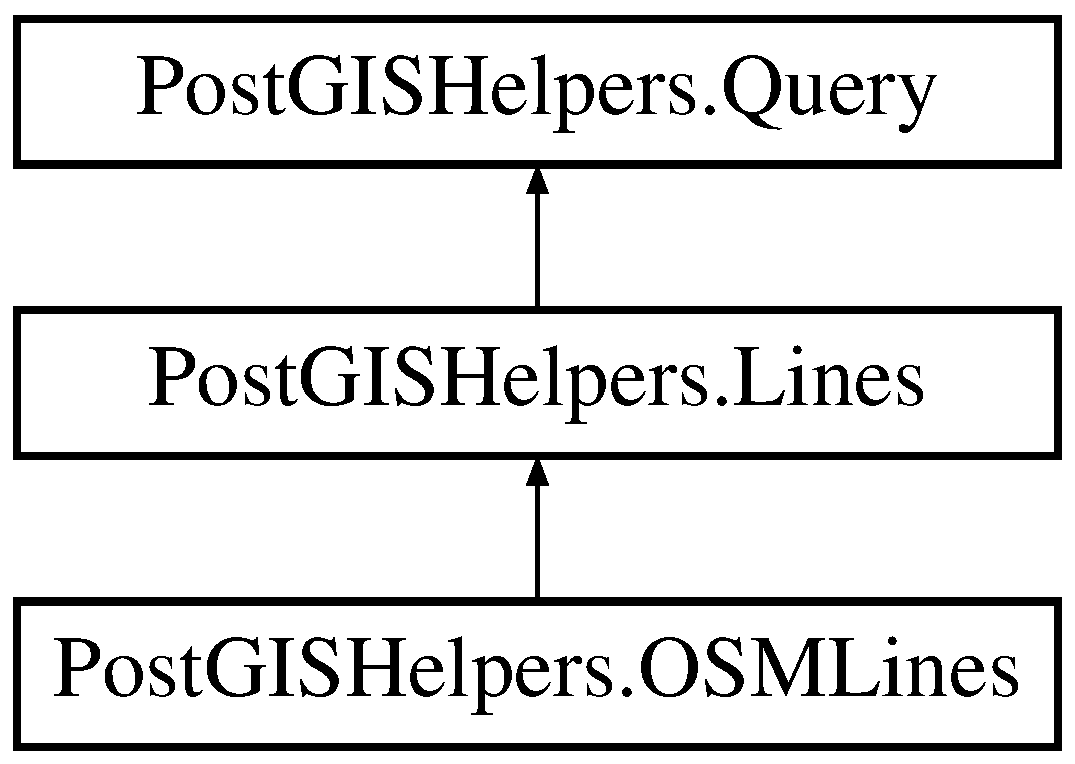
\includegraphics[height=3.000000cm]{class_post_g_i_s_helpers_1_1_lines}
\end{center}
\end{figure}
\subsection*{Public Member Functions}
\begin{DoxyCompactItemize}
\item 
\hypertarget{class_post_g_i_s_helpers_1_1_lines_a994a60bd3368b23dc814b6c5e51bab16}{}def {\bfseries \+\_\+\+\_\+init\+\_\+\+\_\+}\label{class_post_g_i_s_helpers_1_1_lines_a994a60bd3368b23dc814b6c5e51bab16}

\end{DoxyCompactItemize}
\subsection*{Public Attributes}
\begin{DoxyCompactItemize}
\item 
\hypertarget{class_post_g_i_s_helpers_1_1_lines_ad29e175daa61407737beea9117cc23b7}{}{\bfseries geom\+\_\+type}\label{class_post_g_i_s_helpers_1_1_lines_ad29e175daa61407737beea9117cc23b7}

\end{DoxyCompactItemize}
\subsection*{Additional Inherited Members}


The documentation for this class was generated from the following file\+:\begin{DoxyCompactItemize}
\item 
/\+Users/blubber/\+Documents/\+Software\+Dev Workspace/\+Python/\+Projects/rli\+\_\+python\+\_\+as\+\_\+gis/Post\+G\+I\+S\+Helpers.\+py\end{DoxyCompactItemize}

\hypertarget{class_post_g_i_s_helpers_1_1_o_s_m_collection}{}\section{Post\+G\+I\+S\+Helpers.\+O\+S\+M\+Collection Class Reference}
\label{class_post_g_i_s_helpers_1_1_o_s_m_collection}\index{Post\+G\+I\+S\+Helpers.\+O\+S\+M\+Collection@{Post\+G\+I\+S\+Helpers.\+O\+S\+M\+Collection}}
Inheritance diagram for Post\+G\+I\+S\+Helpers.\+O\+S\+M\+Collection\+:\begin{figure}[H]
\begin{center}
\leavevmode
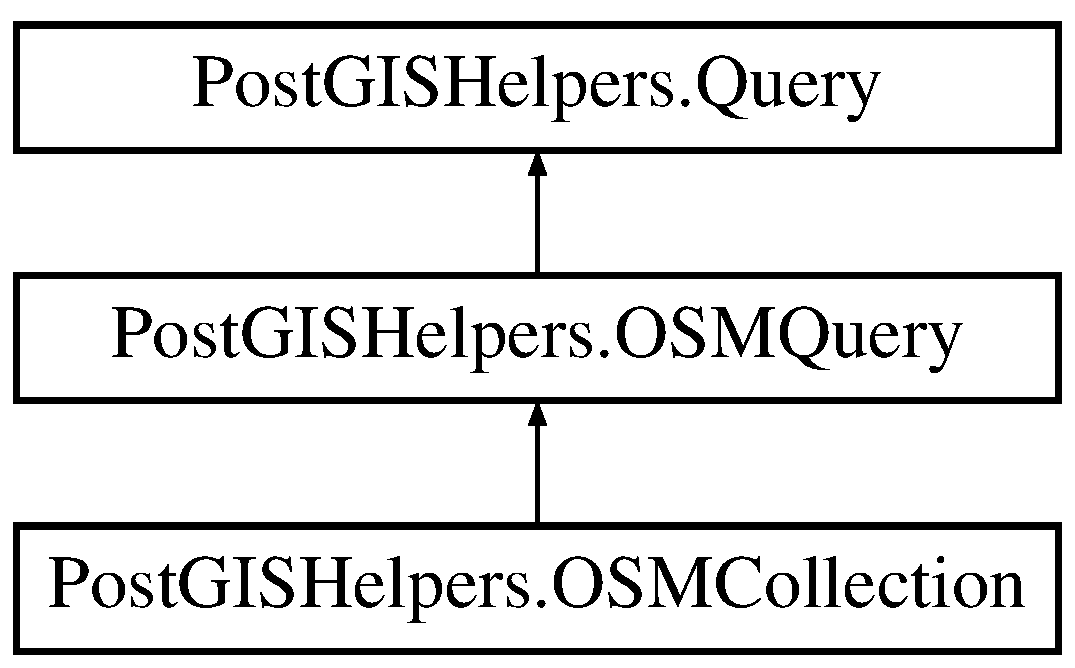
\includegraphics[height=3.000000cm]{class_post_g_i_s_helpers_1_1_o_s_m_collection}
\end{center}
\end{figure}
\subsection*{Public Member Functions}
\begin{DoxyCompactItemize}
\item 
\hypertarget{class_post_g_i_s_helpers_1_1_o_s_m_collection_a52bcf3a425fb5dd150a7c6c2efe0424b}{}def {\bfseries \+\_\+\+\_\+init\+\_\+\+\_\+}\label{class_post_g_i_s_helpers_1_1_o_s_m_collection_a52bcf3a425fb5dd150a7c6c2efe0424b}

\item 
def \hyperlink{class_post_g_i_s_helpers_1_1_o_s_m_collection_af97c78e59020dafe7f277b828adf8d6e}{create\+\_\+collection\+\_\+query}
\item 
def \hyperlink{class_post_g_i_s_helpers_1_1_o_s_m_collection_ae422d255640aa558aa826f4a30e8aeb1}{fetch\+\_\+\+O\+S\+M\+\_\+collection} (self, source\+\_\+db)
\item 
def \hyperlink{class_post_g_i_s_helpers_1_1_o_s_m_collection_ae505c01a43a32c63bba81f7b1424bc11}{plot\+\_\+view}
\end{DoxyCompactItemize}
\subsection*{Public Attributes}
\begin{DoxyCompactItemize}
\item 
\hypertarget{class_post_g_i_s_helpers_1_1_o_s_m_collection_a7f602b55a1c663ef35833377d674f613}{}{\bfseries Points}\label{class_post_g_i_s_helpers_1_1_o_s_m_collection_a7f602b55a1c663ef35833377d674f613}

\item 
\hypertarget{class_post_g_i_s_helpers_1_1_o_s_m_collection_a6fe91065cd9b09252963c2097227341c}{}{\bfseries Lines}\label{class_post_g_i_s_helpers_1_1_o_s_m_collection_a6fe91065cd9b09252963c2097227341c}

\item 
\hypertarget{class_post_g_i_s_helpers_1_1_o_s_m_collection_aac7591e4a09ba35e2e68fcf63bc761fa}{}{\bfseries Polygons}\label{class_post_g_i_s_helpers_1_1_o_s_m_collection_aac7591e4a09ba35e2e68fcf63bc761fa}

\end{DoxyCompactItemize}
\subsection*{Additional Inherited Members}


\subsection{Member Function Documentation}
\hypertarget{class_post_g_i_s_helpers_1_1_o_s_m_collection_af97c78e59020dafe7f277b828adf8d6e}{}\index{Post\+G\+I\+S\+Helpers\+::\+O\+S\+M\+Collection@{Post\+G\+I\+S\+Helpers\+::\+O\+S\+M\+Collection}!create\+\_\+collection\+\_\+query@{create\+\_\+collection\+\_\+query}}
\index{create\+\_\+collection\+\_\+query@{create\+\_\+collection\+\_\+query}!Post\+G\+I\+S\+Helpers\+::\+O\+S\+M\+Collection@{Post\+G\+I\+S\+Helpers\+::\+O\+S\+M\+Collection}}
\subsubsection[{create\+\_\+collection\+\_\+query}]{\setlength{\rightskip}{0pt plus 5cm}def Post\+G\+I\+S\+Helpers.\+O\+S\+M\+Collection.\+create\+\_\+collection\+\_\+query (
\begin{DoxyParamCaption}
\item[{}]{self, }
\item[{}]{relation\+\_\+prefix, }
\item[{}]{schema = {\ttfamily \char`\"{}public\char`\"{}}, }
\item[{}]{select\+\_\+cols = {\ttfamily \char`\"{}$\ast$\char`\"{}}, }
\item[{}]{geom\+\_\+col = {\ttfamily \textquotesingle{}way\textquotesingle{}}, }
\item[{}]{where\+\_\+cond = {\ttfamily None}, }
\item[{}]{S\+R\+I\+D = {\ttfamily 4326}}
\end{DoxyParamCaption}
)}\label{class_post_g_i_s_helpers_1_1_o_s_m_collection_af97c78e59020dafe7f277b828adf8d6e}
\begin{DoxyVerb}Automatically generate and set a collective select/from/where SQL
statement from given query features for a collection of OSMPoints and/or
OSMLines and/or OSMPolygons
:param schema: DB schema to query
:param relation_prefix: OSM table name prefix (suffix is being added
automatically)
:param select_cols: Table columns to select from
:param where_cond: Where condition for query
:param geom_col: Column containing geometries
:param SRID: Spatial Reference ID
\end{DoxyVerb}
 \hypertarget{class_post_g_i_s_helpers_1_1_o_s_m_collection_ae422d255640aa558aa826f4a30e8aeb1}{}\index{Post\+G\+I\+S\+Helpers\+::\+O\+S\+M\+Collection@{Post\+G\+I\+S\+Helpers\+::\+O\+S\+M\+Collection}!fetch\+\_\+\+O\+S\+M\+\_\+collection@{fetch\+\_\+\+O\+S\+M\+\_\+collection}}
\index{fetch\+\_\+\+O\+S\+M\+\_\+collection@{fetch\+\_\+\+O\+S\+M\+\_\+collection}!Post\+G\+I\+S\+Helpers\+::\+O\+S\+M\+Collection@{Post\+G\+I\+S\+Helpers\+::\+O\+S\+M\+Collection}}
\subsubsection[{fetch\+\_\+\+O\+S\+M\+\_\+collection(self, source\+\_\+db)}]{\setlength{\rightskip}{0pt plus 5cm}def Post\+G\+I\+S\+Helpers.\+O\+S\+M\+Collection.\+fetch\+\_\+\+O\+S\+M\+\_\+collection (
\begin{DoxyParamCaption}
\item[{}]{self, }
\item[{}]{source\+\_\+db}
\end{DoxyParamCaption}
)}\label{class_post_g_i_s_helpers_1_1_o_s_m_collection_ae422d255640aa558aa826f4a30e8aeb1}
\begin{DoxyVerb}Collectively fetch OSMCollection containing Points and/or Lines and/or
Polygons
:param source_db: DB to fetch data from
:return:
\end{DoxyVerb}
 \hypertarget{class_post_g_i_s_helpers_1_1_o_s_m_collection_ae505c01a43a32c63bba81f7b1424bc11}{}\index{Post\+G\+I\+S\+Helpers\+::\+O\+S\+M\+Collection@{Post\+G\+I\+S\+Helpers\+::\+O\+S\+M\+Collection}!plot\+\_\+view@{plot\+\_\+view}}
\index{plot\+\_\+view@{plot\+\_\+view}!Post\+G\+I\+S\+Helpers\+::\+O\+S\+M\+Collection@{Post\+G\+I\+S\+Helpers\+::\+O\+S\+M\+Collection}}
\subsubsection[{plot\+\_\+view}]{\setlength{\rightskip}{0pt plus 5cm}def Post\+G\+I\+S\+Helpers.\+O\+S\+M\+Collection.\+plot\+\_\+view (
\begin{DoxyParamCaption}
\item[{}]{self, }
\item[{}]{resolution = {\ttfamily \textquotesingle{}i\textquotesingle{}}, }
\item[{}]{el\+\_\+limit = {\ttfamily 5000}}
\end{DoxyParamCaption}
)}\label{class_post_g_i_s_helpers_1_1_o_s_m_collection_ae505c01a43a32c63bba81f7b1424bc11}
\begin{DoxyVerb}METHOD OVERRIDING: Plot collected geometries of OSMCollection
:param resolution: Set basemap resolution / area threshold that shall
still be displayed
:param el_limit: Maximum number of elements to display on map
\end{DoxyVerb}
 

The documentation for this class was generated from the following file\+:\begin{DoxyCompactItemize}
\item 
/\+Users/blubber/\+Documents/\+Software\+Dev Workspace/\+Python/\+Projects/rli\+\_\+python\+\_\+as\+\_\+gis/Post\+G\+I\+S\+Helpers.\+py\end{DoxyCompactItemize}

\hypertarget{class_post_g_i_s_helpers_1_1_o_s_m_lines}{}\section{Post\+G\+I\+S\+Helpers.\+O\+S\+M\+Lines Class Reference}
\label{class_post_g_i_s_helpers_1_1_o_s_m_lines}\index{Post\+G\+I\+S\+Helpers.\+O\+S\+M\+Lines@{Post\+G\+I\+S\+Helpers.\+O\+S\+M\+Lines}}
Inheritance diagram for Post\+G\+I\+S\+Helpers.\+O\+S\+M\+Lines\+:\begin{figure}[H]
\begin{center}
\leavevmode
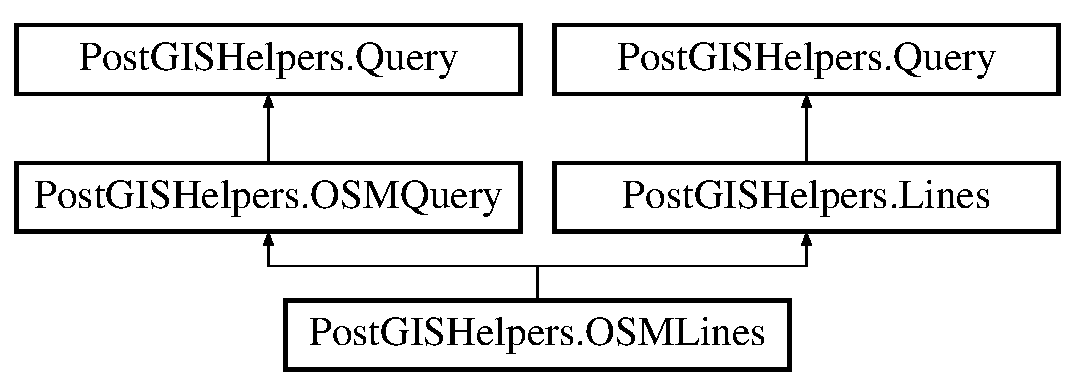
\includegraphics[height=3.000000cm]{class_post_g_i_s_helpers_1_1_o_s_m_lines}
\end{center}
\end{figure}
\subsection*{Public Member Functions}
\begin{DoxyCompactItemize}
\item 
\hypertarget{class_post_g_i_s_helpers_1_1_o_s_m_lines_accee2f90f93b9b068f7999fadd147d49}{}def {\bfseries \+\_\+\+\_\+init\+\_\+\+\_\+}\label{class_post_g_i_s_helpers_1_1_o_s_m_lines_accee2f90f93b9b068f7999fadd147d49}

\end{DoxyCompactItemize}
\subsection*{Additional Inherited Members}


The documentation for this class was generated from the following file\+:\begin{DoxyCompactItemize}
\item 
/\+Users/blubber/\+Documents/\+Software\+Dev Workspace/\+Python/\+Projects/rli\+\_\+python\+\_\+as\+\_\+gis/Post\+G\+I\+S\+Helpers.\+py\end{DoxyCompactItemize}

\hypertarget{class_post_g_i_s_helpers_1_1_o_s_m_points}{}\section{Post\+G\+I\+S\+Helpers.\+O\+S\+M\+Points Class Reference}
\label{class_post_g_i_s_helpers_1_1_o_s_m_points}\index{Post\+G\+I\+S\+Helpers.\+O\+S\+M\+Points@{Post\+G\+I\+S\+Helpers.\+O\+S\+M\+Points}}
Inheritance diagram for Post\+G\+I\+S\+Helpers.\+O\+S\+M\+Points\+:\begin{figure}[H]
\begin{center}
\leavevmode
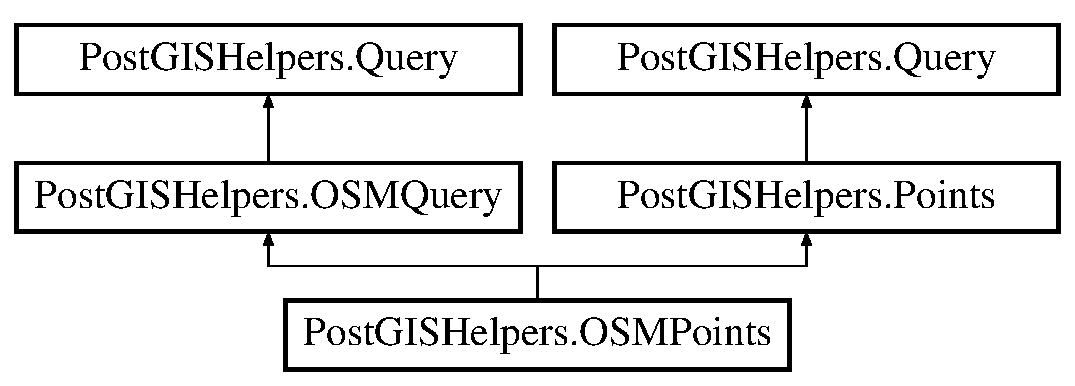
\includegraphics[height=3.000000cm]{class_post_g_i_s_helpers_1_1_o_s_m_points}
\end{center}
\end{figure}
\subsection*{Public Member Functions}
\begin{DoxyCompactItemize}
\item 
\hypertarget{class_post_g_i_s_helpers_1_1_o_s_m_points_a0a00cdc88ad4057b455e4221a8674c90}{}def {\bfseries \+\_\+\+\_\+init\+\_\+\+\_\+}\label{class_post_g_i_s_helpers_1_1_o_s_m_points_a0a00cdc88ad4057b455e4221a8674c90}

\end{DoxyCompactItemize}
\subsection*{Additional Inherited Members}


The documentation for this class was generated from the following file\+:\begin{DoxyCompactItemize}
\item 
/\+Users/blubber/\+Documents/\+Software\+Dev Workspace/\+Python/\+Projects/rli\+\_\+python\+\_\+as\+\_\+gis/Post\+G\+I\+S\+Helpers.\+py\end{DoxyCompactItemize}

\hypertarget{class_post_g_i_s_helpers_1_1_o_s_m_polygons}{}\section{Post\+G\+I\+S\+Helpers.\+O\+S\+M\+Polygons Class Reference}
\label{class_post_g_i_s_helpers_1_1_o_s_m_polygons}\index{Post\+G\+I\+S\+Helpers.\+O\+S\+M\+Polygons@{Post\+G\+I\+S\+Helpers.\+O\+S\+M\+Polygons}}
Inheritance diagram for Post\+G\+I\+S\+Helpers.\+O\+S\+M\+Polygons\+:\begin{figure}[H]
\begin{center}
\leavevmode
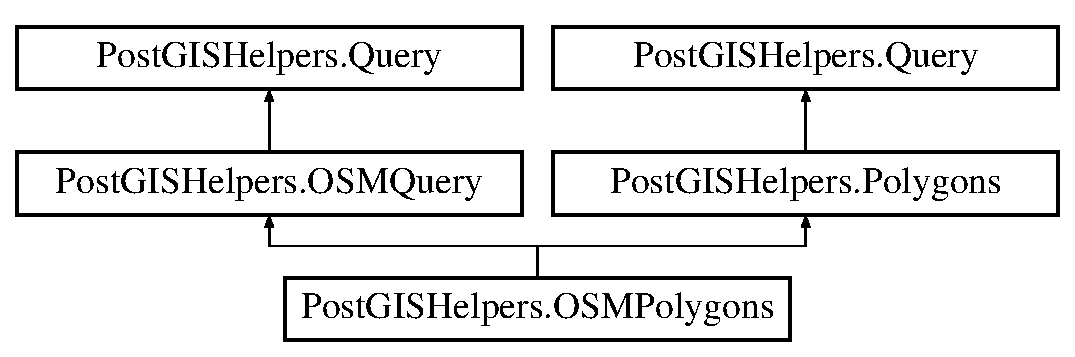
\includegraphics[height=3.000000cm]{class_post_g_i_s_helpers_1_1_o_s_m_polygons}
\end{center}
\end{figure}
\subsection*{Public Member Functions}
\begin{DoxyCompactItemize}
\item 
\hypertarget{class_post_g_i_s_helpers_1_1_o_s_m_polygons_a79bddc2532ce28deef345ad80a6dfc4a}{}def {\bfseries \+\_\+\+\_\+init\+\_\+\+\_\+}\label{class_post_g_i_s_helpers_1_1_o_s_m_polygons_a79bddc2532ce28deef345ad80a6dfc4a}

\end{DoxyCompactItemize}
\subsection*{Additional Inherited Members}


The documentation for this class was generated from the following file\+:\begin{DoxyCompactItemize}
\item 
/\+Users/blubber/\+Documents/\+Software\+Dev Workspace/\+Python/\+Projects/rli\+\_\+python\+\_\+as\+\_\+gis/Post\+G\+I\+S\+Helpers.\+py\end{DoxyCompactItemize}

\hypertarget{class_post_g_i_s_helpers_1_1_o_s_m_query}{}\section{Post\+G\+I\+S\+Helpers.\+O\+S\+M\+Query Class Reference}
\label{class_post_g_i_s_helpers_1_1_o_s_m_query}\index{Post\+G\+I\+S\+Helpers.\+O\+S\+M\+Query@{Post\+G\+I\+S\+Helpers.\+O\+S\+M\+Query}}
Inheritance diagram for Post\+G\+I\+S\+Helpers.\+O\+S\+M\+Query\+:\begin{figure}[H]
\begin{center}
\leavevmode
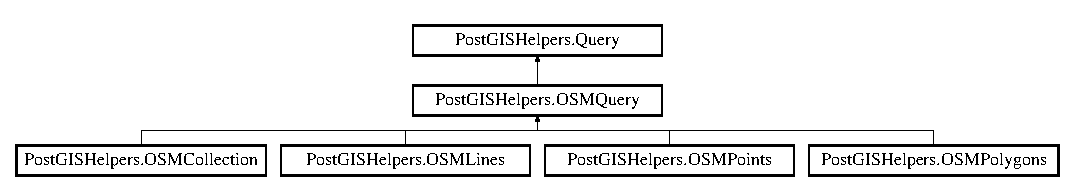
\includegraphics[height=2.131979cm]{class_post_g_i_s_helpers_1_1_o_s_m_query}
\end{center}
\end{figure}
\subsection*{Public Member Functions}
\begin{DoxyCompactItemize}
\item 
\hypertarget{class_post_g_i_s_helpers_1_1_o_s_m_query_a3c279dbb90bb1cfad3321f36adbba0ec}{}def {\bfseries \+\_\+\+\_\+init\+\_\+\+\_\+}\label{class_post_g_i_s_helpers_1_1_o_s_m_query_a3c279dbb90bb1cfad3321f36adbba0ec}

\end{DoxyCompactItemize}
\subsection*{Additional Inherited Members}


The documentation for this class was generated from the following file\+:\begin{DoxyCompactItemize}
\item 
/\+Users/blubber/\+Documents/\+Software\+Dev Workspace/\+Python/\+Projects/rli\+\_\+python\+\_\+as\+\_\+gis/Post\+G\+I\+S\+Helpers.\+py\end{DoxyCompactItemize}

\hypertarget{class_post_g_i_s_helpers_1_1_points}{}\section{Post\+G\+I\+S\+Helpers.\+Points Class Reference}
\label{class_post_g_i_s_helpers_1_1_points}\index{Post\+G\+I\+S\+Helpers.\+Points@{Post\+G\+I\+S\+Helpers.\+Points}}
Inheritance diagram for Post\+G\+I\+S\+Helpers.\+Points\+:\begin{figure}[H]
\begin{center}
\leavevmode
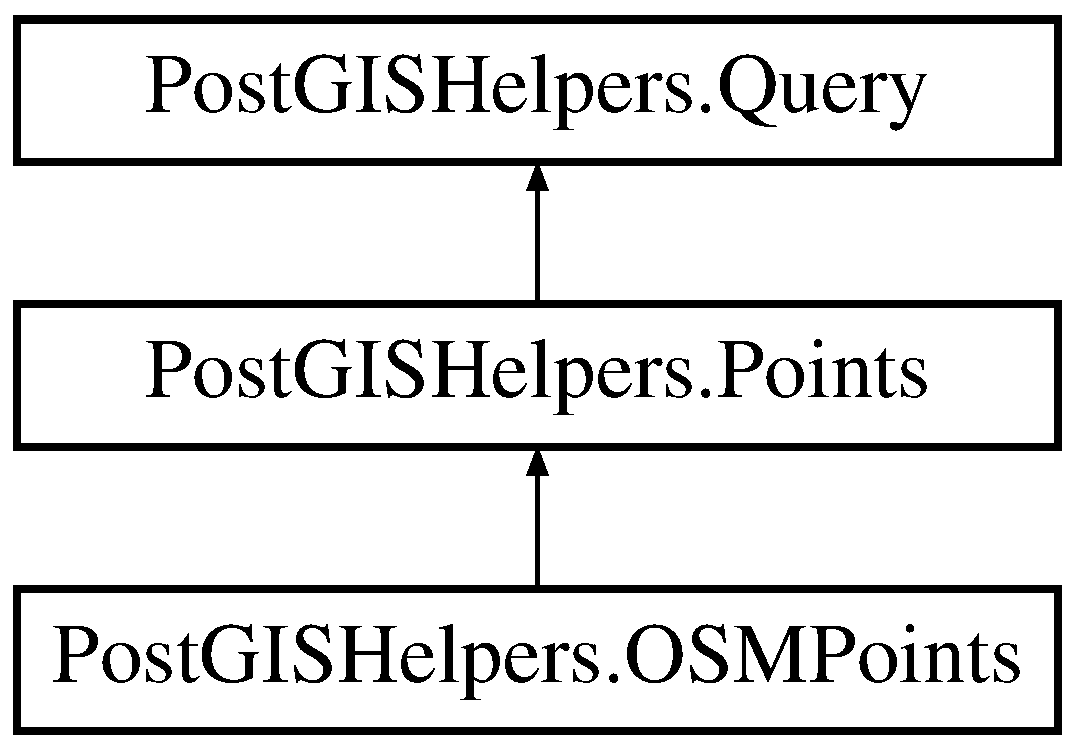
\includegraphics[height=3.000000cm]{class_post_g_i_s_helpers_1_1_points}
\end{center}
\end{figure}
\subsection*{Public Member Functions}
\begin{DoxyCompactItemize}
\item 
\hypertarget{class_post_g_i_s_helpers_1_1_points_ab686c6e368a48a99940b8fd55492e4ea}{}def {\bfseries \+\_\+\+\_\+init\+\_\+\+\_\+}\label{class_post_g_i_s_helpers_1_1_points_ab686c6e368a48a99940b8fd55492e4ea}

\end{DoxyCompactItemize}
\subsection*{Public Attributes}
\begin{DoxyCompactItemize}
\item 
\hypertarget{class_post_g_i_s_helpers_1_1_points_a7682483b6cbcd543c99472de72d07baf}{}{\bfseries geom\+\_\+type}\label{class_post_g_i_s_helpers_1_1_points_a7682483b6cbcd543c99472de72d07baf}

\end{DoxyCompactItemize}
\subsection*{Additional Inherited Members}


The documentation for this class was generated from the following file\+:\begin{DoxyCompactItemize}
\item 
/\+Users/blubber/\+Documents/\+Software\+Dev Workspace/\+Python/\+Projects/rli\+\_\+python\+\_\+as\+\_\+gis/Post\+G\+I\+S\+Helpers.\+py\end{DoxyCompactItemize}

\hypertarget{class_post_g_i_s_helpers_1_1_polygons}{}\section{Post\+G\+I\+S\+Helpers.\+Polygons Class Reference}
\label{class_post_g_i_s_helpers_1_1_polygons}\index{Post\+G\+I\+S\+Helpers.\+Polygons@{Post\+G\+I\+S\+Helpers.\+Polygons}}
Inheritance diagram for Post\+G\+I\+S\+Helpers.\+Polygons\+:\begin{figure}[H]
\begin{center}
\leavevmode
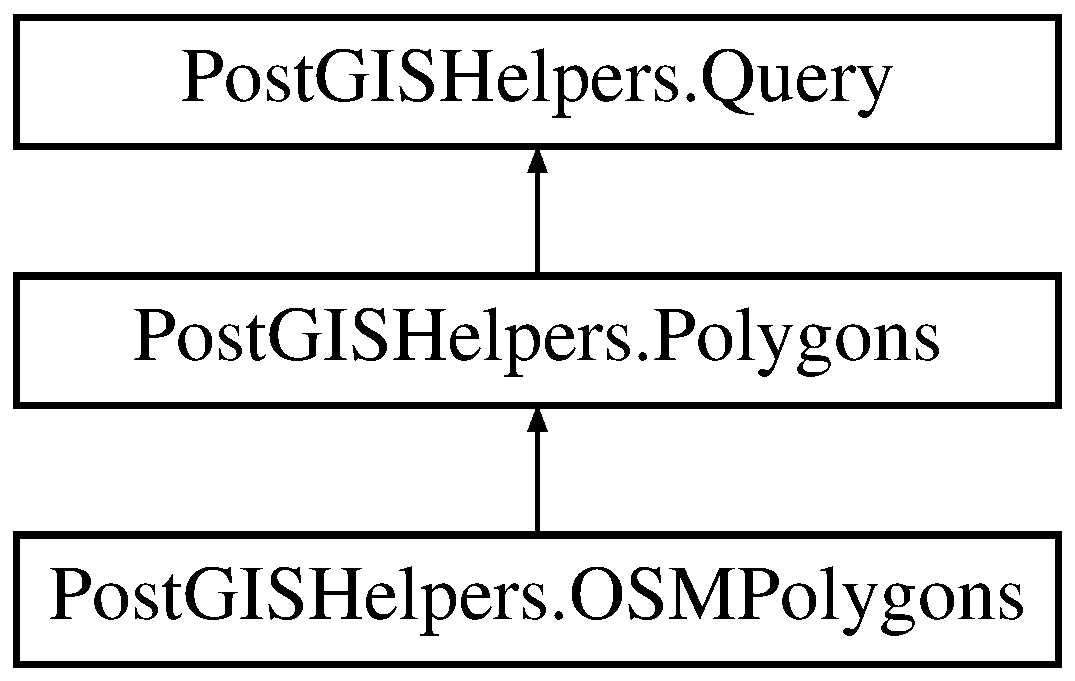
\includegraphics[height=3.000000cm]{class_post_g_i_s_helpers_1_1_polygons}
\end{center}
\end{figure}
\subsection*{Public Member Functions}
\begin{DoxyCompactItemize}
\item 
\hypertarget{class_post_g_i_s_helpers_1_1_polygons_a77591d8421e5d6296fb75b7e5b30eb9d}{}def {\bfseries \+\_\+\+\_\+init\+\_\+\+\_\+}\label{class_post_g_i_s_helpers_1_1_polygons_a77591d8421e5d6296fb75b7e5b30eb9d}

\item 
def \hyperlink{class_post_g_i_s_helpers_1_1_polygons_a510ea7ccacca4a6158164e06d6a2bb87}{area\+\_\+sum} (self)
\end{DoxyCompactItemize}
\subsection*{Public Attributes}
\begin{DoxyCompactItemize}
\item 
\hypertarget{class_post_g_i_s_helpers_1_1_polygons_a0edee8c1382c28d0d16b28e8d267c950}{}{\bfseries geom\+\_\+type}\label{class_post_g_i_s_helpers_1_1_polygons_a0edee8c1382c28d0d16b28e8d267c950}

\end{DoxyCompactItemize}
\subsection*{Additional Inherited Members}


\subsection{Member Function Documentation}
\hypertarget{class_post_g_i_s_helpers_1_1_polygons_a510ea7ccacca4a6158164e06d6a2bb87}{}\index{Post\+G\+I\+S\+Helpers\+::\+Polygons@{Post\+G\+I\+S\+Helpers\+::\+Polygons}!area\+\_\+sum@{area\+\_\+sum}}
\index{area\+\_\+sum@{area\+\_\+sum}!Post\+G\+I\+S\+Helpers\+::\+Polygons@{Post\+G\+I\+S\+Helpers\+::\+Polygons}}
\subsubsection[{area\+\_\+sum(self)}]{\setlength{\rightskip}{0pt plus 5cm}def Post\+G\+I\+S\+Helpers.\+Polygons.\+area\+\_\+sum (
\begin{DoxyParamCaption}
\item[{}]{self}
\end{DoxyParamCaption}
)}\label{class_post_g_i_s_helpers_1_1_polygons_a510ea7ccacca4a6158164e06d6a2bb87}
\begin{DoxyVerb}:rtype : float
Calculate area of polygons in Polygons()
:return: Sum of polygon areas
\end{DoxyVerb}
 

The documentation for this class was generated from the following file\+:\begin{DoxyCompactItemize}
\item 
/\+Users/blubber/\+Documents/\+Software\+Dev Workspace/\+Python/\+Projects/rli\+\_\+python\+\_\+as\+\_\+gis/Post\+G\+I\+S\+Helpers.\+py\end{DoxyCompactItemize}

\hypertarget{class_post_g_i_s_helpers_1_1_query}{}\section{Post\+G\+I\+S\+Helpers.\+Query Class Reference}
\label{class_post_g_i_s_helpers_1_1_query}\index{Post\+G\+I\+S\+Helpers.\+Query@{Post\+G\+I\+S\+Helpers.\+Query}}
Inheritance diagram for Post\+G\+I\+S\+Helpers.\+Query\+:\begin{figure}[H]
\begin{center}
\leavevmode
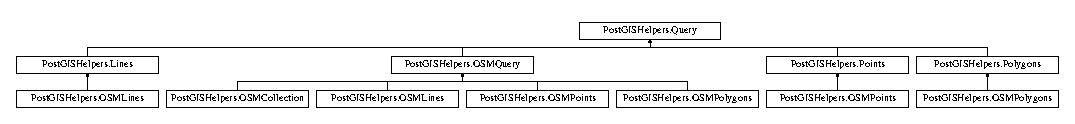
\includegraphics[height=1.218274cm]{class_post_g_i_s_helpers_1_1_query}
\end{center}
\end{figure}
\subsection*{Public Member Functions}
\begin{DoxyCompactItemize}
\item 
\hypertarget{class_post_g_i_s_helpers_1_1_query_ae91481a4425fa5e713348e50de2b64da}{}def {\bfseries \+\_\+\+\_\+init\+\_\+\+\_\+}\label{class_post_g_i_s_helpers_1_1_query_ae91481a4425fa5e713348e50de2b64da}

\item 
def \hyperlink{class_post_g_i_s_helpers_1_1_query_a7b15a1e1045d7d422f00973e7995b9b7}{create\+\_\+where\+\_\+query}
\item 
def \hyperlink{class_post_g_i_s_helpers_1_1_query_a74b5b36b5b55e68b46243e80138706ab}{insert\+\_\+custom\+\_\+query} (self, query\+\_\+text)
\item 
def \hyperlink{class_post_g_i_s_helpers_1_1_query_a8cc7e86f8de045e5d96cc79676d3b273}{clip\+\_\+view2poly} (self)
\item 
def \hyperlink{class_post_g_i_s_helpers_1_1_query_a4812c3452ebfc2e42fe5d2d49c276ea4}{string2psycopg\+\_\+features} (self, db\+\_\+string)
\item 
def \hyperlink{class_post_g_i_s_helpers_1_1_query_aef1b7806337023919a4c21028f957f55}{fetch\+\_\+geoms} (self, source\+\_\+db)
\item 
def \hyperlink{class_post_g_i_s_helpers_1_1_query_a061572cc1f94289ea6ed18e029a39d11}{print\+\_\+results}
\item 
def \hyperlink{class_post_g_i_s_helpers_1_1_query_aab94f519185f5427498d8d672f80955a}{bbox\+\_\+of\+\_\+view} (self, results)
\item 
def \hyperlink{class_post_g_i_s_helpers_1_1_query_abe2e937630c1271f306721fffe1a133a}{plot\+\_\+view}
\item 
def \hyperlink{class_post_g_i_s_helpers_1_1_query_a21579a5070811c493975b6ac34b82672}{export2shp} (self, filepath)
\end{DoxyCompactItemize}
\subsection*{Public Attributes}
\begin{DoxyCompactItemize}
\item 
\hypertarget{class_post_g_i_s_helpers_1_1_query_a706d7d70a7066397321be865498d00c6}{}{\bfseries query\+\_\+name}\label{class_post_g_i_s_helpers_1_1_query_a706d7d70a7066397321be865498d00c6}

\item 
\hypertarget{class_post_g_i_s_helpers_1_1_query_a34878bb3f66d0c82bcb69b230740bb60}{}{\bfseries results}\label{class_post_g_i_s_helpers_1_1_query_a34878bb3f66d0c82bcb69b230740bb60}

\item 
\hypertarget{class_post_g_i_s_helpers_1_1_query_ab927b3006bc5811d25032d2c437fb7f1}{}{\bfseries region}\label{class_post_g_i_s_helpers_1_1_query_ab927b3006bc5811d25032d2c437fb7f1}

\item 
\hypertarget{class_post_g_i_s_helpers_1_1_query_ad62d93aec6d82a9fc4c6163e565455f5}{}{\bfseries geom\+\_\+type}\label{class_post_g_i_s_helpers_1_1_query_ad62d93aec6d82a9fc4c6163e565455f5}

\item 
\hypertarget{class_post_g_i_s_helpers_1_1_query_a854bc699b4b841227568bf0828a95f67}{}{\bfseries S\+R\+I\+D}\label{class_post_g_i_s_helpers_1_1_query_a854bc699b4b841227568bf0828a95f67}

\item 
\hypertarget{class_post_g_i_s_helpers_1_1_query_a0f712cbb6791002bdd57b12e2a1c14a9}{}{\bfseries select\+\_\+cols}\label{class_post_g_i_s_helpers_1_1_query_a0f712cbb6791002bdd57b12e2a1c14a9}

\end{DoxyCompactItemize}
\subsection*{Static Public Attributes}
\begin{DoxyCompactItemize}
\item 
\hypertarget{class_post_g_i_s_helpers_1_1_query_afb80ded1f2426bcc599c70c497578e03}{}dictionary {\bfseries instances} = \{\}\label{class_post_g_i_s_helpers_1_1_query_afb80ded1f2426bcc599c70c497578e03}

\end{DoxyCompactItemize}


\subsection{Member Function Documentation}
\hypertarget{class_post_g_i_s_helpers_1_1_query_aab94f519185f5427498d8d672f80955a}{}\index{Post\+G\+I\+S\+Helpers\+::\+Query@{Post\+G\+I\+S\+Helpers\+::\+Query}!bbox\+\_\+of\+\_\+view@{bbox\+\_\+of\+\_\+view}}
\index{bbox\+\_\+of\+\_\+view@{bbox\+\_\+of\+\_\+view}!Post\+G\+I\+S\+Helpers\+::\+Query@{Post\+G\+I\+S\+Helpers\+::\+Query}}
\subsubsection[{bbox\+\_\+of\+\_\+view(self, results)}]{\setlength{\rightskip}{0pt plus 5cm}def Post\+G\+I\+S\+Helpers.\+Query.\+bbox\+\_\+of\+\_\+view (
\begin{DoxyParamCaption}
\item[{}]{self, }
\item[{}]{results}
\end{DoxyParamCaption}
)}\label{class_post_g_i_s_helpers_1_1_query_aab94f519185f5427498d8d672f80955a}
\begin{DoxyVerb}Calculate the bounding box of query results if no further regional
information have been supplied (Region.bounds = None)
:rtype : dict
:param results: return dict of fetch_geoms(...)
:return: bbox dict {'xmin':float, 'xmax':float, ...}
\end{DoxyVerb}
 \hypertarget{class_post_g_i_s_helpers_1_1_query_a8cc7e86f8de045e5d96cc79676d3b273}{}\index{Post\+G\+I\+S\+Helpers\+::\+Query@{Post\+G\+I\+S\+Helpers\+::\+Query}!clip\+\_\+view2poly@{clip\+\_\+view2poly}}
\index{clip\+\_\+view2poly@{clip\+\_\+view2poly}!Post\+G\+I\+S\+Helpers\+::\+Query@{Post\+G\+I\+S\+Helpers\+::\+Query}}
\subsubsection[{clip\+\_\+view2poly(self)}]{\setlength{\rightskip}{0pt plus 5cm}def Post\+G\+I\+S\+Helpers.\+Query.\+clip\+\_\+view2poly (
\begin{DoxyParamCaption}
\item[{}]{self}
\end{DoxyParamCaption}
)}\label{class_post_g_i_s_helpers_1_1_query_a8cc7e86f8de045e5d96cc79676d3b273}
\begin{DoxyVerb}Clips list of n-tuples as result of SELECT-query to boundary of a given
instance of Region()
\end{DoxyVerb}
 \hypertarget{class_post_g_i_s_helpers_1_1_query_a7b15a1e1045d7d422f00973e7995b9b7}{}\index{Post\+G\+I\+S\+Helpers\+::\+Query@{Post\+G\+I\+S\+Helpers\+::\+Query}!create\+\_\+where\+\_\+query@{create\+\_\+where\+\_\+query}}
\index{create\+\_\+where\+\_\+query@{create\+\_\+where\+\_\+query}!Post\+G\+I\+S\+Helpers\+::\+Query@{Post\+G\+I\+S\+Helpers\+::\+Query}}
\subsubsection[{create\+\_\+where\+\_\+query}]{\setlength{\rightskip}{0pt plus 5cm}def Post\+G\+I\+S\+Helpers.\+Query.\+create\+\_\+where\+\_\+query (
\begin{DoxyParamCaption}
\item[{}]{self, }
\item[{}]{relation, }
\item[{}]{schema = {\ttfamily \char`\"{}public\char`\"{}}, }
\item[{}]{select\+\_\+cols = {\ttfamily \char`\"{}$\ast$\char`\"{}}, }
\item[{}]{geom\+\_\+col = {\ttfamily \textquotesingle{}way\textquotesingle{}}, }
\item[{}]{where\+\_\+cond = {\ttfamily None}, }
\item[{}]{S\+R\+I\+D = {\ttfamily 4326}}
\end{DoxyParamCaption}
)}\label{class_post_g_i_s_helpers_1_1_query_a7b15a1e1045d7d422f00973e7995b9b7}
\begin{DoxyVerb}Automatically generate and set a select/from/where SQL statement
from given query features
:param schema: DB schema to query
:param relation: table name
:param select_cols: table columns to select from
:param where_cond: where condition for query
:param SRID: Spatial Reference ID
\end{DoxyVerb}
 \hypertarget{class_post_g_i_s_helpers_1_1_query_a21579a5070811c493975b6ac34b82672}{}\index{Post\+G\+I\+S\+Helpers\+::\+Query@{Post\+G\+I\+S\+Helpers\+::\+Query}!export2shp@{export2shp}}
\index{export2shp@{export2shp}!Post\+G\+I\+S\+Helpers\+::\+Query@{Post\+G\+I\+S\+Helpers\+::\+Query}}
\subsubsection[{export2shp(self, filepath)}]{\setlength{\rightskip}{0pt plus 5cm}def Post\+G\+I\+S\+Helpers.\+Query.\+export2shp (
\begin{DoxyParamCaption}
\item[{}]{self, }
\item[{}]{filepath}
\end{DoxyParamCaption}
)}\label{class_post_g_i_s_helpers_1_1_query_a21579a5070811c493975b6ac34b82672}
\begin{DoxyVerb}Save results to hard disk
:param filepath: output path
\end{DoxyVerb}
 \hypertarget{class_post_g_i_s_helpers_1_1_query_aef1b7806337023919a4c21028f957f55}{}\index{Post\+G\+I\+S\+Helpers\+::\+Query@{Post\+G\+I\+S\+Helpers\+::\+Query}!fetch\+\_\+geoms@{fetch\+\_\+geoms}}
\index{fetch\+\_\+geoms@{fetch\+\_\+geoms}!Post\+G\+I\+S\+Helpers\+::\+Query@{Post\+G\+I\+S\+Helpers\+::\+Query}}
\subsubsection[{fetch\+\_\+geoms(self, source\+\_\+db)}]{\setlength{\rightskip}{0pt plus 5cm}def Post\+G\+I\+S\+Helpers.\+Query.\+fetch\+\_\+geoms (
\begin{DoxyParamCaption}
\item[{}]{self, }
\item[{}]{source\+\_\+db}
\end{DoxyParamCaption}
)}\label{class_post_g_i_s_helpers_1_1_query_aef1b7806337023919a4c21028f957f55}
\begin{DoxyVerb}Fetches items from PostGIS DB and clips results to boundary of supplied
Region object instance
:param source_db: String containing information on where to fetch data
from
:return : List of dictionary with keys 'geom' (containing WKT-formatted
geometries) and '
\end{DoxyVerb}
 \hypertarget{class_post_g_i_s_helpers_1_1_query_a74b5b36b5b55e68b46243e80138706ab}{}\index{Post\+G\+I\+S\+Helpers\+::\+Query@{Post\+G\+I\+S\+Helpers\+::\+Query}!insert\+\_\+custom\+\_\+query@{insert\+\_\+custom\+\_\+query}}
\index{insert\+\_\+custom\+\_\+query@{insert\+\_\+custom\+\_\+query}!Post\+G\+I\+S\+Helpers\+::\+Query@{Post\+G\+I\+S\+Helpers\+::\+Query}}
\subsubsection[{insert\+\_\+custom\+\_\+query(self, query\+\_\+text)}]{\setlength{\rightskip}{0pt plus 5cm}def Post\+G\+I\+S\+Helpers.\+Query.\+insert\+\_\+custom\+\_\+query (
\begin{DoxyParamCaption}
\item[{}]{self, }
\item[{}]{query\+\_\+text}
\end{DoxyParamCaption}
)}\label{class_post_g_i_s_helpers_1_1_query_a74b5b36b5b55e68b46243e80138706ab}
\begin{DoxyVerb}Set custom SQL statement
:param query_text:
\end{DoxyVerb}
 \hypertarget{class_post_g_i_s_helpers_1_1_query_abe2e937630c1271f306721fffe1a133a}{}\index{Post\+G\+I\+S\+Helpers\+::\+Query@{Post\+G\+I\+S\+Helpers\+::\+Query}!plot\+\_\+view@{plot\+\_\+view}}
\index{plot\+\_\+view@{plot\+\_\+view}!Post\+G\+I\+S\+Helpers\+::\+Query@{Post\+G\+I\+S\+Helpers\+::\+Query}}
\subsubsection[{plot\+\_\+view}]{\setlength{\rightskip}{0pt plus 5cm}def Post\+G\+I\+S\+Helpers.\+Query.\+plot\+\_\+view (
\begin{DoxyParamCaption}
\item[{}]{self, }
\item[{}]{resolution = {\ttfamily \textquotesingle{}i\textquotesingle{}}, }
\item[{}]{el\+\_\+limit = {\ttfamily 5000}}
\end{DoxyParamCaption}
)}\label{class_post_g_i_s_helpers_1_1_query_abe2e937630c1271f306721fffe1a133a}
\begin{DoxyVerb}Show map of fetched geometries
:param resolution: Set basemap resolution / area threshold that shall
still be displayed
:param el_limit: Maximum number of elements to display on map
\end{DoxyVerb}
 \hypertarget{class_post_g_i_s_helpers_1_1_query_a061572cc1f94289ea6ed18e029a39d11}{}\index{Post\+G\+I\+S\+Helpers\+::\+Query@{Post\+G\+I\+S\+Helpers\+::\+Query}!print\+\_\+results@{print\+\_\+results}}
\index{print\+\_\+results@{print\+\_\+results}!Post\+G\+I\+S\+Helpers\+::\+Query@{Post\+G\+I\+S\+Helpers\+::\+Query}}
\subsubsection[{print\+\_\+results}]{\setlength{\rightskip}{0pt plus 5cm}def Post\+G\+I\+S\+Helpers.\+Query.\+print\+\_\+results (
\begin{DoxyParamCaption}
\item[{}]{self, }
\item[{}]{n = {\ttfamily 1000}}
\end{DoxyParamCaption}
)}\label{class_post_g_i_s_helpers_1_1_query_a061572cc1f94289ea6ed18e029a39d11}
\begin{DoxyVerb}Print fetched results as nicely formatted table
:param n: Limit of result rows to display
\end{DoxyVerb}
 \hypertarget{class_post_g_i_s_helpers_1_1_query_a4812c3452ebfc2e42fe5d2d49c276ea4}{}\index{Post\+G\+I\+S\+Helpers\+::\+Query@{Post\+G\+I\+S\+Helpers\+::\+Query}!string2psycopg\+\_\+features@{string2psycopg\+\_\+features}}
\index{string2psycopg\+\_\+features@{string2psycopg\+\_\+features}!Post\+G\+I\+S\+Helpers\+::\+Query@{Post\+G\+I\+S\+Helpers\+::\+Query}}
\subsubsection[{string2psycopg\+\_\+features(self, db\+\_\+string)}]{\setlength{\rightskip}{0pt plus 5cm}def Post\+G\+I\+S\+Helpers.\+Query.\+string2psycopg\+\_\+features (
\begin{DoxyParamCaption}
\item[{}]{self, }
\item[{}]{db\+\_\+string}
\end{DoxyParamCaption}
)}\label{class_post_g_i_s_helpers_1_1_query_a4812c3452ebfc2e42fe5d2d49c276ea4}
\begin{DoxyVerb}Convert input string containing DB access information in SQLAlchemy
style format ('user@host:port/database-name')
:rtype : dict
:return : dictionary of DB access information
\end{DoxyVerb}
 

The documentation for this class was generated from the following file\+:\begin{DoxyCompactItemize}
\item 
/\+Users/blubber/\+Documents/\+Software\+Dev Workspace/\+Python/\+Projects/rli\+\_\+python\+\_\+as\+\_\+gis/Post\+G\+I\+S\+Helpers.\+py\end{DoxyCompactItemize}

\hypertarget{classregion_1_1_region}{}\section{region.\+Region Class Reference}
\label{classregion_1_1_region}\index{region.\+Region@{region.\+Region}}
\subsection*{Public Member Functions}
\begin{DoxyCompactItemize}
\item 
\hypertarget{classregion_1_1_region_a5481ca1f882d196c24cb5876a9dd17b7}{}def {\bfseries \+\_\+\+\_\+init\+\_\+\+\_\+}\label{classregion_1_1_region_a5481ca1f882d196c24cb5876a9dd17b7}

\item 
def \hyperlink{classregion_1_1_region_ab010509ab92699cce3a29584b5bfbf87}{set\+\_\+boundaries} (self, boundary)
\end{DoxyCompactItemize}
\subsection*{Public Attributes}
\begin{DoxyCompactItemize}
\item 
\hypertarget{classregion_1_1_region_a1acb0c939379ea8bfdc5407214ab5444}{}{\bfseries name}\label{classregion_1_1_region_a1acb0c939379ea8bfdc5407214ab5444}

\item 
\hypertarget{classregion_1_1_region_acbfb565824f33820de559559b5c1cf87}{}{\bfseries boundary\+\_\+polygon}\label{classregion_1_1_region_acbfb565824f33820de559559b5c1cf87}

\item 
\hypertarget{classregion_1_1_region_a3ddcfe9b0f68ab5f4dce9eed39ae369d}{}{\bfseries bounds}\label{classregion_1_1_region_a3ddcfe9b0f68ab5f4dce9eed39ae369d}

\end{DoxyCompactItemize}
\subsection*{Static Public Attributes}
\begin{DoxyCompactItemize}
\item 
\hypertarget{classregion_1_1_region_ad6e627f3c120cf1fbfec6b40b771c760}{}dictionary {\bfseries instances} = \{\}\label{classregion_1_1_region_ad6e627f3c120cf1fbfec6b40b771c760}

\end{DoxyCompactItemize}


\subsection{Detailed Description}
\begin{DoxyVerb}Define region object, instances can be passed to Query() in order to set
boundaries for queries in a PostGIS-DB
\end{DoxyVerb}
 

\subsection{Member Function Documentation}
\hypertarget{classregion_1_1_region_ab010509ab92699cce3a29584b5bfbf87}{}\index{region\+::\+Region@{region\+::\+Region}!set\+\_\+boundaries@{set\+\_\+boundaries}}
\index{set\+\_\+boundaries@{set\+\_\+boundaries}!region\+::\+Region@{region\+::\+Region}}
\subsubsection[{set\+\_\+boundaries(self, boundary)}]{\setlength{\rightskip}{0pt plus 5cm}def region.\+Region.\+set\+\_\+boundaries (
\begin{DoxyParamCaption}
\item[{}]{self, }
\item[{}]{boundary}
\end{DoxyParamCaption}
)}\label{classregion_1_1_region_ab010509ab92699cce3a29584b5bfbf87}
\begin{DoxyVerb}Set boundary bbox
:return:
\end{DoxyVerb}
 

The documentation for this class was generated from the following file\+:\begin{DoxyCompactItemize}
\item 
/\+Users/blubber/\+Documents/\+Software\+Dev Workspace/\+Python/\+Projects/rli\+\_\+python\+\_\+as\+\_\+gis/region.\+py\end{DoxyCompactItemize}

\hypertarget{classsimple__log_1_1_simple_logger}{}\section{simple\+\_\+log.\+Simple\+Logger Class Reference}
\label{classsimple__log_1_1_simple_logger}\index{simple\+\_\+log.\+Simple\+Logger@{simple\+\_\+log.\+Simple\+Logger}}
\subsection*{Public Member Functions}
\begin{DoxyCompactItemize}
\item 
\hypertarget{classsimple__log_1_1_simple_logger_adf6f4a11fe20be4cc9ca700a2ee8e816}{}def {\bfseries \+\_\+\+\_\+init\+\_\+\+\_\+}\label{classsimple__log_1_1_simple_logger_adf6f4a11fe20be4cc9ca700a2ee8e816}

\item 
def \hyperlink{classsimple__log_1_1_simple_logger_a716f168beed60164e9d2ccd6e7111412}{set\+\_\+debug\+\_\+level} (self, value)
\end{DoxyCompactItemize}
\subsection*{Public Attributes}
\begin{DoxyCompactItemize}
\item 
\hypertarget{classsimple__log_1_1_simple_logger_ab97878571701a768a09b5c2b96f45995}{}{\bfseries printmessage}\label{classsimple__log_1_1_simple_logger_ab97878571701a768a09b5c2b96f45995}

\end{DoxyCompactItemize}
\subsection*{Static Public Attributes}
\begin{DoxyCompactItemize}
\item 
\hypertarget{classsimple__log_1_1_simple_logger_a14da51c0946b94047d1c54e92a97b196}{}int {\bfseries logging\+\_\+status} = 0\label{classsimple__log_1_1_simple_logger_a14da51c0946b94047d1c54e92a97b196}

\end{DoxyCompactItemize}


\subsection{Member Function Documentation}
\hypertarget{classsimple__log_1_1_simple_logger_a716f168beed60164e9d2ccd6e7111412}{}\index{simple\+\_\+log\+::\+Simple\+Logger@{simple\+\_\+log\+::\+Simple\+Logger}!set\+\_\+debug\+\_\+level@{set\+\_\+debug\+\_\+level}}
\index{set\+\_\+debug\+\_\+level@{set\+\_\+debug\+\_\+level}!simple\+\_\+log\+::\+Simple\+Logger@{simple\+\_\+log\+::\+Simple\+Logger}}
\subsubsection[{set\+\_\+debug\+\_\+level(self, value)}]{\setlength{\rightskip}{0pt plus 5cm}def simple\+\_\+log.\+Simple\+Logger.\+set\+\_\+debug\+\_\+level (
\begin{DoxyParamCaption}
\item[{}]{self, }
\item[{}]{value}
\end{DoxyParamCaption}
)}\label{classsimple__log_1_1_simple_logger_a716f168beed60164e9d2ccd6e7111412}
\begin{DoxyVerb}Set level of logging output to either
('d', 10): 'debug':
('i', 20): 'info'
('w', 30): 'warning'
('r', 40): 'error'
('c', 50): 'critical'
:param value: Debug level from 10-50
\end{DoxyVerb}
 

The documentation for this class was generated from the following file\+:\begin{DoxyCompactItemize}
\item 
/\+Users/blubber/\+Documents/\+Software\+Dev Workspace/\+Python/\+Projects/rli\+\_\+python\+\_\+as\+\_\+gis/simple\+\_\+log.\+py\end{DoxyCompactItemize}

%--- End generated contents ---

% Index
\backmatter
\newpage
\phantomsection
\clearemptydoublepage
\addcontentsline{toc}{chapter}{Index}
\printindex

\end{document}
